\begin{table}
\begin{center}
\Large
文档历史发放及记录\vspace{3ex}\\
\scriptsize
\begin{tabular}{|c|c|c|c|c|c|}
\hline
序号 & 变更(+/-说明) & 作者 & 版本号 & 日期 & 批准 \\
\hline  
1 & 创建 & 钟志威 & V0.1 & 2018/7/27 &  \\
\hline
2 & 修改(+PPAPI历史、注册、生命周期) & 钟志威 & V0.2 & 2018/8/2 & \\
\hline
\end{tabular}
\end{center}
\end{table}
\clearpage

%---------------------------------------------------------------------

\renewcommand{\contentsname}{\hspace*{\fill}目\quad 录\hspace*{\fill}}
\tableofcontents

%---------------------------------------------------------------------

\vspace{50ex}
\section{引言}
\subsection{插件历史}
插件一直是浏览器的重要组成部分,实现一些HTML+JS实现不了本地应用(比如音视频、文件操作等)。\par
早期IE发布的插件ActiveX,它基于COM规范,在IE占浏览器市场主流份额的时代,银行开发网页安全控件都是使用ActiveX开发。
虽然ActiveX出尽了风头,但它并不是浏览器业内的插件标准,由网景发布的NPAPI是除了IE之外的其他浏览器共同支持的业内标准。\par
现在,随着IE逐渐退出历史舞台,ActiveX插件的运行范围越来越窄。而NPAPI插件定义的API接口太旧且易用性差,崩溃和安全问题也很多,
无法适应现代浏览器的发展。虽然很多银行已经支持NPAPI版本的安全控件,但NPAPI却做为不安全因素被主流浏览器(Chrome、FireFox)抛弃。\par
Google从2012年,基于NPAPI自主研发了一套API接口,称为PPAPI接口,全称是Pepper Plugin API。相比于NPAPI,PPAPI接口封装得更完善,开发更方便,
且运行在Chrome的沙箱模型里,安全性得到保证。从2014年起,Chrome逐渐放弃对NPAPI插件的支持,因此本文接下来要分析的是PPAPI插件。

\subsection{开发背景}
目前海外产品需要支持hbbtv和netrange两业务,而支持这两业务必须实现其插件。以前tbrowser1.0和tbrowser2.0分别使用NPAPI去实现
插件,而最新的tbrowser2.61已经不再支持NPAPI,使用的则是PPAPI。本文旨在介绍PPAPI的加载流程和使用方法,供开发人员参考。

\subsection{软件名称}
PPAPI插件\quad——\quad 由Google自主研发的浏览器插件系统

\subsection{术语和缩略语}
\begin{center}
\begin{tabular}{ccc}
\hline
缩略语/术语 & 全\quad 称 & 说\quad 明 \\  
\hline
PPAPI & Pepper Plugin Application Programming Interface & \\
\hline
\end{tabular}
\end{center}

\subsection{参考资料}
https://blog.csdn.net/luoshengyang/article/details/48417255 \par
https://blog.csdn.net/wbsong1978/article/details/77658912 \par
https://code.google.com/p/ppapi/wiki/InterfacingWithJavaScript

%---------------------------------------------------------------------

\section{总体设计}
\subsection{需求规定}
\begin{enumerate}
\item 对HTML的embed和object标签插件的支持
\item 支持创建插件并由页面调用到其自定义的属性和方法
\end{enumerate}

\subsection{运行环境}
Linux

\subsection{上下文定义}
\begin{figure}[H] 
  \centering 
  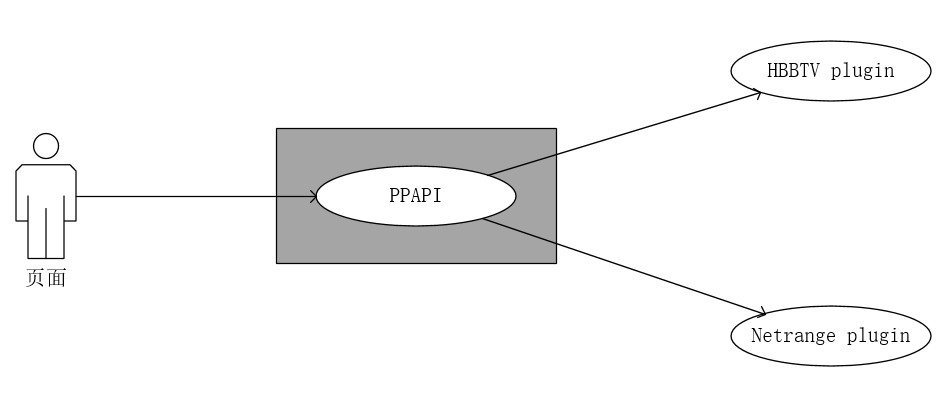
\includegraphics[width=\textwidth]{image/ppapi/use_case.jpg} 
  \caption{PPAPI插件上下文} 
\end{figure}

\vspace{10ex}
\begin{center}
\begin{tabular}{|c|c|}
\hline
功能模块 & 说明 \\
\hline  
页面 & 使用object或者embed标签的HTML页面 \\
\hline
PPAPI & Google自主研发的插件系统 \\
\hline
Netrange Plugin & Netrange插件实现 \\
\hline
HBBTV Plugin & HBBTV插件实现 \\
\hline
\end{tabular}
\end{center}

\subsection{PPAPI插件进程与其他进程关系图}
\begin{figure}[H] 
  \centering 
  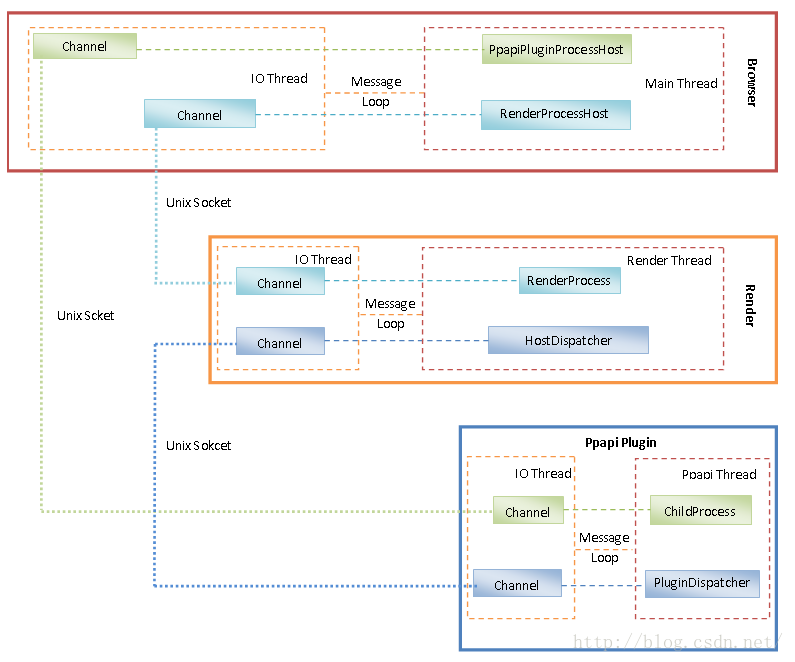
\includegraphics[width=\textwidth]{image/ppapi/process.jpg} 
  \caption{PPAPI插件进程与Browser进程、Render进程的关系}
  \label{process_jpg}
\end{figure}

如图~\ref{process_jpg}所示:
Render进程在解析网页时,如果遇到一个object标签,那么就会创建一个HTMLPlugInElement对象来描述该标签,
并且调用该HTMLPlugInElement对象的成员函数loadPlugin加载对应的PPAPI插件。但是Render进程没有启动PPAPI插件进程的权限,
因此它就会通过之前与Browser进程建立的IPC通道向Browser进程发出一个启动PPAPI插件进程的请求。\par
Browser进程接收到启动PPAPI插件进程的请求之后,就会启动一个PPAPI插件进程,并且创建一个PpapiPluginProcessHost对象描述该PPAPI插件进程。
PPAPI插件进程启动起来之后,会在内部创建一个ChildProcess对象,用来与Browser进程中的PpapiPluginProcessHost对象建立一个IPC通道。\par
有了这个IPC通道之后,Browser进程请求PPAPI插件进程创建另外一个UINX Socket。该UNIX Socket的Server端文件描述符保留在PPAPI进程中,
Client端文件描述符则返回给Render进程。基于这个UNIX Socket的Server端和Client端文件描述符,PPAPI插件进程和Render进程将分别创建
一个HostDispatcher对象和一个PluginDispatcher对象,构成一个Plugin通道。以后PPAPI插件进程和Render进程就通过该Plugin通道进行通信。

%---------------------------------------------------------------------

\section{运行设计}
\subsection{注册PPAPI插件}
chromium注册插件默认是通过register-pepper-plugins启动命令传给浏览器并保存在PepperPluginInfo类里,示例如下:\\
\begin{spacing}{1.0}
\begin{lstlisting}[language={C++}]
--register-pepper-plugins="/data/tbrowser2.61/plugins/libdemo_plugin.so;application/demo_plugin;application/demo_plugin1,/data/tbrowser2.61/plugins/libutil.so;application/util"
\end{lstlisting}
\end{spacing}
首先,多个PPAPI插件进程以","为间隔,我们称一个PPAPI插件进程对应一个plugin\_module。\par
接着,一个plugin\_module以";"为间隔,第一个参数代表PPAPI插件动态库的路径,后面的参数表示PPAPI插件的type类型,可以有多个。 \par
换而言之,一个PPAPI插件动态库对应一个PPAPI插件进程,PPAPI插件动态库与PPAPI插件类型可以是一对一,也可以是一对多的关系(详情可见插件之基于C++的实现)。\par
最后,pepper\_plugin\_list.cc文件里描述了register-pepper-plugins具体参数格式:
\begin{spacing}{1.0}
\begin{lstlisting}[language={C++}]
command-line = <plugin-entry> + *( LWS + "," + LWS + <plugin-entry> ) 
plugin-entry =
  <file-path> +
  ["#" + <name> + ["#" + <description> + ["#" + <version>]]] +
  *1( LWS + ";" + LWS + <mime-type-data> )
mime-type-data = <mime-type> + [ LWS + "#" + LWS + <extension> ]
\end{lstlisting}
\end{spacing}

\subsection{PPAPI插件生命周期}
以单个插件库为例,当页面检测到有object标签,且type与之前注册的type匹配,插件进程就会启动,并且会创建一个pp::Module实例。\\
\begin{spacing}{1.0}
\begin{lstlisting}[language={C++}]
<object id="pluginId" type="application/demo_plugin"></object>
<object id="pluginId1" type="application/demo_plugin1"></object>
\end{lstlisting}
\end{spacing}
此时页面检测到两个object标签,pp::Module实例就会创建两个pp::Instance的实例,一一对应。当其中一个object标签被删除的时候,对应的pp::Instance
类实例就被析构。当最后一个object标签被删除时,对应的pp::Instance的实例也被析构。此时,页面已无object标签,在plugin\_process\_dispatcher.cc文件里
有一个kPluginReleaseTimeSeconds整型变量,值为30,其含义是在30s之内,如果页面还是没有创建新的对应该进程插件type的object标签,pp::Module类就会被析构,
插件进程也会退出。当再次检测到有object标签时,重复上过程。

\subsection{实现PPAPI Plugin}
基于PPAPI机制实现的插件有C和C++两种实现。

\subsubsection{基于C的实现}
无论是可信的还是不可信的PPAPI组件,一般都会提供三个导出函数:
\begin{spacing}{1.0}
\begin{lstlisting}[language={C++}]
// @brief 初始化PPAPI模块
// @param[in] module 传入浏览器生成的模块句柄PP_Module 
// @param[in] get_browser_interface 给插件模块提供浏览器宿主常见的功能的函数指针接口,比如PPB_Core、
// PPB_Messaging 、PPB_URLLoader、PPB_FileIO等接口。
// @return 返回PP_OK表示成功,其他都为失败
int32_t PPP_InitializeModule(PP_Module module, PPB_GetInterface get_browser_interface);
\end{lstlisting}
\end{spacing}

\begin{spacing}{1.0}
\begin{lstlisting}[language={C++}]
// @brief 关闭PPAPI模块
void PPP_ShutdownModule(void);
\end{lstlisting}
\end{spacing}

\begin{spacing}{1.0}
\begin{lstlisting}[language={C++}]
// @brief 提供给浏览器的插件功能接口
// @param[in] interface_name 提供给浏览器的插件功能接口字符串,比如PPP_Instance、PPP_InputEvent、PPP_Messaging
// 等接口
// @return 返回这个接口的指针,返回NULL表示无此接口
const void* PPP_GetInterface(const char* interface_name);
\end{lstlisting}
\end{spacing}

{\color{red}注:除了PPP\_ShutdownModule是可选的,其他两个导出函数必须实现。PPB\_GetInterface
和PPP\_GetInterface是插件(PPAPI)和宿主(浏览器的Plugin进程)功能交互的唯一
切入口。}

\vspace{5ex}
命名规范上,宿主Browser提供给插件(PPAPI)的接口以PPB命名开头,可以从导出
函数PPP\_InitializeModule 传入的PPB\_GetInterface参数中根据接口ID查询对应的功
能接口,下面列举一些常用的功能接口:
\begin{center}
\scriptsize
\begin{tabular}{|l|p{5cm}|p{3cm}|p{5cm}|}
\hline
功能说明 & 接口ID & 接口定义 & 重要成员方法说明 \\
\hline  
核心基础接口 & PPB\_CORE\_INTERFACE & PPB\_Core & AddRefResource、ReleaseResource:增加/减少资源的引用计数GetTime、GetTimeTicks:获取当前的时间CallOnMainThread、IsMainThread:主线程相关的处理 \\
\hline
消息接口 & PPB\_MESSAGING\_INTERFACE & PPB\_Messaging & PostMessage:抛送消息(Plugin->JS,JS通过addEventListener挂接message事件)
RegisterMessageHandler、UnregisterMessageHandler:自定义消息处理对象,用于拦截PPP\_Messaging接口的HandleMessage处理(应用场景未明)\\
\hline
HTTP请求接口 & PPB\_URLLOADER\_INTERFACE & PPB\_URLLoader & 常用的HTTP请求操作:Open、GetResponseInfo、ReadResponseBody、Close等等 \\
\hline
文件IO操作 & PPB\_FILEIO\_INTERFACE & PPB\_FileIO & File的基本操作:Create、Open、Read、Write、Close等 \\
\hline
网络操作 & PPB\_UDPSOCKET\_INTERFACE PPB\_TCPSOCKET\_INTERFACE PPB\_HOSTRESOLVER\_INTERFACE等
& PPB\_UDPSocket PPB\_TCPSocket PPB\_HostResolver等
& UDP套接字、TCP套接字、域名解析服务等常用的操作接口 \\
\hline
音视频操作 & PPB\_AUDIO\_INTERFACE PPB\_VIDEODECODER\_INTERFACE PPB\_VIDEOENCODER\_INTERFACE等
& PPB\_Audio PPB\_VideoDecoder PPB\_VideoEncoder等
& 封装音视频的编解码等操作 \\
\hline
\end{tabular}
\end{center}
此外还有Image、2D、3D等接口,基本上满足开发本地应用的所有功能。

\clearpage
插件(PPAPI)提供给宿主Browser的接口以PPP命名开头:
\begin{center}
\scriptsize
\begin{tabular}{|l|p{5cm}|p{3cm}|p{5cm}|}
\hline
功能说明 & 接口ID & 接口定义 & 重要成员方法说明 \\
\hline  
插件实例对象 & PPP\_INSTANCE\_INTERFACE & PPP\_Instance & DidCreate、DidDestroy:插件创建销毁通知;
DidChangeView、DidChangeFocus:插件尺寸、焦点改变通知;
HandleDocumentLoad:Document加载完成通知;
这些调用最终都映射到Instance实例的相关成员方法上
\\
\hline
输入接口 & PPP\_INPUT\_EVENT\_INTERFACE & PPP\_InputEvent & HandleInputEvent:处理输入消息,最终转接到Instance的HandleInputEvent接口 \\
\hline
消息接口 & PPP\_MESSAGING\_INTERFACE & PPP\_Messaging & HandleMessage:处理消息(JS->Plugin, JS调用插件的postMessage方法),最终映射到Instance实例的HandleMessage方法 \\
\hline
\end{tabular}
\end{center}

除了这三个基础的接口,Module对象(后面再细讲)的AddPluginInterface提供了扩展插件接口的功能,比如:\par
封装PDF插件功能的PPP\_Pdf接口;\par
封装视频采集功能的PPP\_VideoCapture\_Dev接口;\par
封装视频硬件解码的PPP\_VideoDecoder\_Dev接口;\par
封装3D图形相关的通知事件的PPP\_Graphics3D接口;\par
此外还有PPP\_MouseLock、PPP\_Find\_Private、PPP\_Instance\_Private等私有接口。

\subsubsection{基于C++的实现}
首先,使用C++版本,开发者就无需关心上述三个导出函数的具体实现,框架在ppp\_entrypoints.cc文件里对三个导出函数做了实现,创建Module对象标识整个插件模块:
\begin{figure}[H] 
  \centering 
  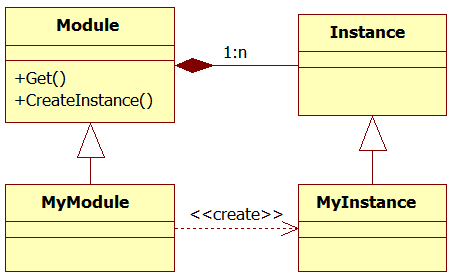
\includegraphics[width=\textwidth]{image/ppapi/ppapi_class.jpg} 
  \caption{ppapi plugin静态类图}
\end{figure}

\vspace{10ex}
开发者只需要提供自己的Module实现MyModule,定制自己的插件实例MyInstance即可,示例代码:
\begin{spacing}{1.0}
\begin{lstlisting}[language={C++}]
class MyInstance : public pp::Instance {
 public:
  explicit MyInstance(PP_Instance instance) : pp::Instance(instance) {}
  virtual ~MyInstance() {}

  virtual bool Init(uint32_t argc, const char* argn[], const char* argv[]) {
    return true;
  }
};

// This object is the global object representing this plugin library as long
// as it is loaded.
class MyModule : public pp::Module {
 public:
  MyModule() : pp::Module() {}
  virtual ~MyModule() {}

  // Override CreateInstance to create your customized Instance object.
  virtual pp::Instance* CreateInstance(PP_Instance instance) {
    return new MyInstance(instance);
  }
};

namespace pp {
// Factory function for your specialization of the Module object.
Module* CreateModule() {
  return new MyModule();
}
}  // namespace pp
\end{lstlisting}
\end{spacing}

\vspace{10ex}
上述实现方式继承了默认的Instance类,该类供页面操作的函数只有HandleMessage和PostMessage方法,
不能使用自定义的方法和属性。如果想使用自定义的属性和方法,还需以下实现方式。
\begin{figure}[H] 
  \centering 
  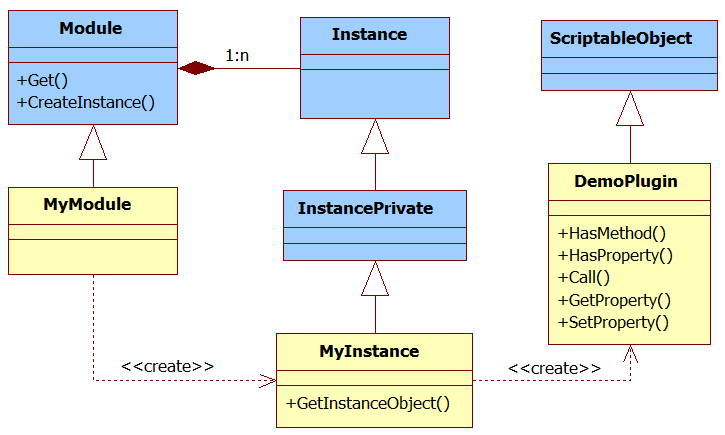
\includegraphics[width=\textwidth]{image/ppapi/ppapi_class1.jpg} 
  \caption{ppapi plugin可自定义方法静态类图}
\end{figure}
代码实现:
\begin{spacing}{1.0}
\begin{lstlisting}[language={C++}]
class DemoPlugin : public pp::deprecated::ScriptableObject {
 public:
  explicit DemoPlugin(pp::InstancePrivate* instance)
      : instance_(instance) {}
  ~DemoPlugin() override {}

  // pp::deprecated::ScriptableObject overrides:
  bool HasMethod(const pp::Var& name, pp::Var* exception) override {
    ...
  }

  bool HasProperty(const pp::Var& name, pp::Var* exception) override {
    ...
  }

  pp::Var Call(const pp::Var& method_name,
               const std::vector<pp::Var>& args,
               pp::Var* exception) override {
    ...
  }

  pp::Var GetProperty(const pp::Var& name, pp::Var* exception) override {
    ...
  }

  void SetProperty(const pp::Var& name,
                   const pp::Var& value,
                   pp::Var* exception) override {
    ...
  }
};


class MyInstance : public pp::InstancePrivate {
 public:
  explicit MyInstance(PP_Instance instance)
      : pp::InstancePrivate(instance) {}
  ~MyInstance() override {}

  // pp::Instance overrides
  bool Init(uint32_t argc, const char* argn[], const char* argv[]) override {
    ...
  }

  virtual bool HandleInputEvent(const pp::InputEvent& event) override {
    ...
  }

  // pp::InstancePrivate overrides:
  pp::Var GetInstanceObject() override {
    if (instance_var_.is_undefined()) {
      instance_ = new DemoPlugin(this);
      instance_var_ = pp::VarPrivate(this, instance_);
    }
    return instance_var_;
  }

 private:
  pp::VarPrivate instance_var_;
};

class MyModule : public pp::Module {
 public:
  MyModule() {}
  ~MyModule() override {}

  virtual pp::Instance* CreateInstance(PP_Instance instance) {
    return new MyInstance(instance);
  }
};

namespace pp {

Module* CreateModule() {
  return new MyModule();
}

}  // namespace pp
\end{lstlisting}
\end{spacing}

\vspace{10ex}
问:如何一个插件动态库可以对应多个插件类型呢?\par
页面:
\begin{spacing}{1.0}
\begin{lstlisting}[language={C++}]
<object id="pluginId" type="application/demo_plugin"></object>
<object id="pluginId1" type="application/demo_plugin1"></object>
\end{lstlisting}
\end{spacing}

由上面页面,假设插件type都匹配上了,那么MyInstance类会创建两个实例,分别执行重写的Init方法。Init方法三个参数含义分别是参数个数、参数key值、参数value值,
其实就是对应上面页面的"id"和"type"。具体实现如下:
\begin{spacing}{1.0}
\begin{lstlisting}[language={C++}]
class MyInstance : public pp::InstancePrivate {
 public:
  explicit MyInstance(PP_Instance instance)
      : pp::InstancePrivate(instance) {}
  ~MyInstance() override {}

  // pp::Instance overrides
  bool Init(uint32_t argc, const char* argn[], const char* argv[]) override {
    if (argc < 1)
      return false;
      
    for (uint32_t i = 0; i < argc; i++) {
      if(std::string(argn[i]) == "type")
        mime_type_ = argv[i];
    }
    return true;
  }

  // pp::InstancePrivate overrides:
  pp::Var GetInstanceObject() override {
    if (instance_var_.is_undefined()) {
      if (mime_type_ == "application/demo_plugin")
        instance_ = new DemoPlugin(this);
      else if (mime_type_ == "application/demo_plugin1")
        instance_ = new DemoPlugin1(this);
      instance_var_ = pp::VarPrivate(this, instance_);
    }
    return instance_var_;
  }

 private:
  pp::VarPrivate instance_var_;
  std::string mime_type_;
};
\end{lstlisting}
\end{spacing}

我们只需要在Init函数的时候保存插件的mimetype值,然后在GetInstanceObject函数的时候,根据mimetype值new相应的插件实现类即可。
%---------------------------------------------------------------------

\section{其他}
\subsection{调用性能对比}
在js中调用插件方法,传递1024字节的字符串到c++代码,连续调用1000次,测试20组数据。使用NPAPI机制平均耗时1658ms;而使用PPAPI机制耗时平均耗时8136ms,经过代码优化后,目前平均耗时2208ms。

\subsection{时序图}
\begin{figure}[H] 
  \centering 
  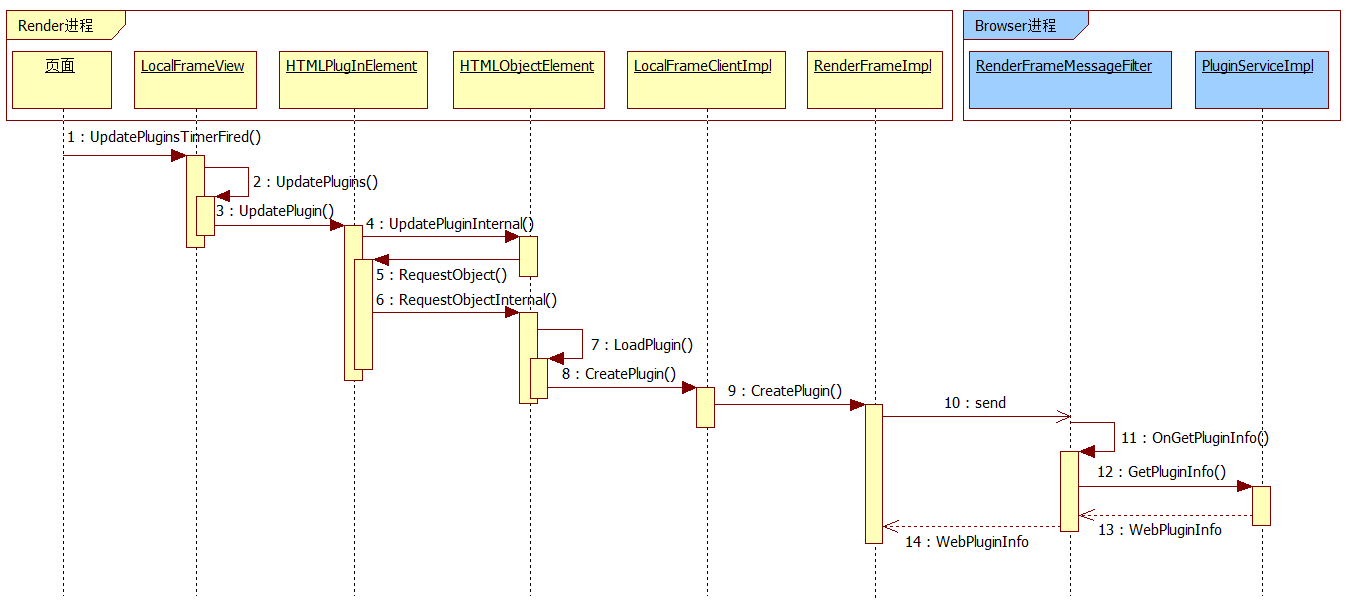
\includegraphics[width=\textwidth]{image/ppapi/ppapi_is_type.jpg} 
  \caption{判断object标签是否存在相应PPAPI插件type时序图}
\end{figure}

\begin{figure}[H] 
  \centering 
  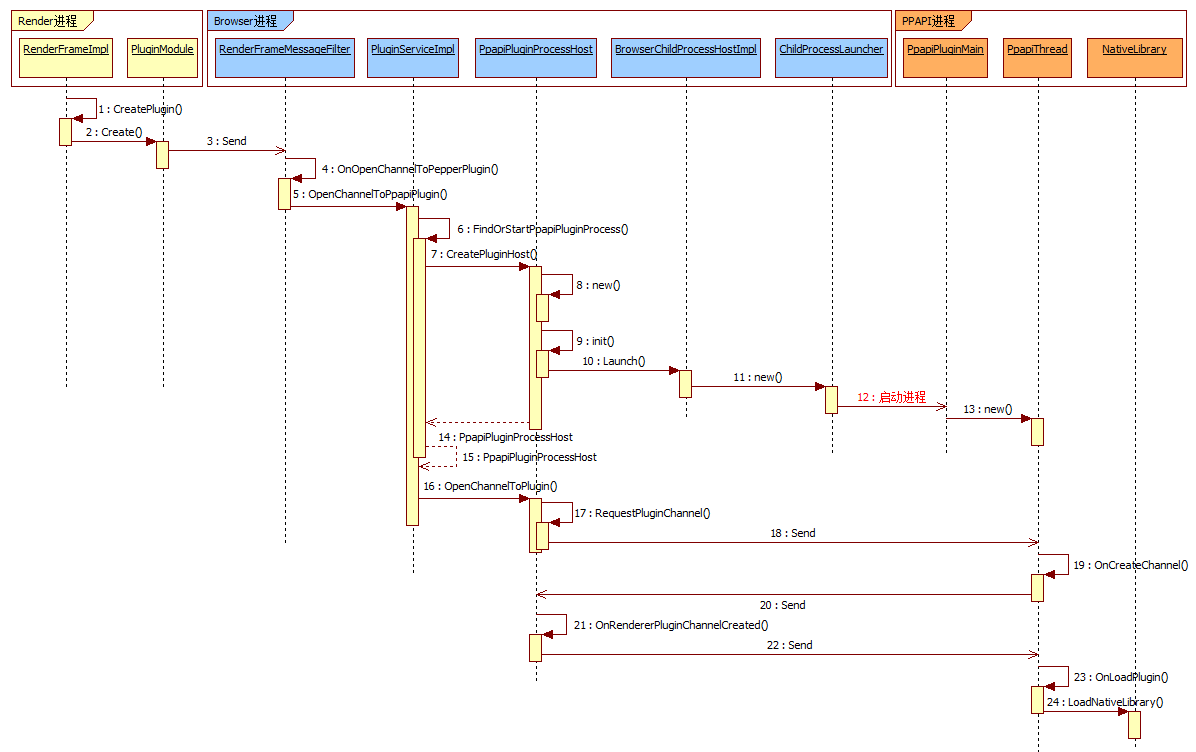
\includegraphics[width=\textwidth]{image/ppapi/ppapi_process.jpg} 
  \caption{PPAPI插件进程启动以及加载插件库时序图}
\end{figure}

%---------------------------------------------------------------------

\ifx\withtbrowser\undefined
\else
\section{Extension Framework使用到的v8 API}

FunctionTemplate类是Function类的模板类,可以理解为设置Function的公共特性,
通过FunctionTemplate类new出来的Function类就拥有这些特性。相当于页面的function。
\begin{spacing}{1.0}
\begin{lstlisting}[language={C++}]
/**
@brief new一个FunctionTemplate对象

@param[in] isolate表示一个独立的v8引擎实例,每个实例维护不同的状态
@param[in] callback是回调函数,创建实例或方法被调用时会调用
@param[in] data表示给回调函数传递的额外的参数
@return 返回FunctionTemplate对象
*/
static Local<FunctionTemplate> New(
    Isolate* isolate, FunctionCallback callback = 0,
    Local<Value> data = Local<Value>(),
    Local<Signature> signature = Local<Signature>(), int length = 0,
    ConstructorBehavior behavior = ConstructorBehavior::kAllow);

/**
 * Set the call-handler callback for a FunctionTemplate.  This
 * callback is called whenever the function created from this
 * FunctionTemplate is called.
 */
void SetCallHandler(FunctionCallback callback,
    Local<Value> data = Local<Value>());
\end{lstlisting}
\end{spacing}

ObjectTemplate类是Object类的模板类,可以理解为设置Object的公共特性,
通过ObjectTemplate类new出来的Object类就拥有这些特性。相当于页面的object。
\begin{spacing}{1.0}
\begin{lstlisting}[language={C++}]
/**
@brief new一个ObjectTemplate对象

@param[in] isolate表示一个独立的v8引擎实例,每个实例维护不同的状态
@param[in] constructor是默认构造函数,只用于创建实例时会调用
@return 返回ObjectTemplate对象
*/
static Local<ObjectTemplate> New(
    Isolate* isolate,
    Local<FunctionTemplate> constructor = Local<FunctionTemplate>());

/**
@brief new一个Object对象实例

@param[in] context表示JavaScript代码运行环境上下文
@return 返回Object对象
*/
V8_WARN_UNUSED_RESULT MaybeLocal<Object> NewInstance(Local<Context> context);

/**
@brief 能够指定JavaScript访问对象属性时的一个callback

@param[in] getter表示获取属性时会被调用的callback
@param[in] setter表示设置属性时会被调用的callback
*/
void SetNamedPropertyHandler(NamedPropertyGetterCallback getter,
    NamedPropertySetterCallback setter = 0,
    NamedPropertyQueryCallback query = 0,
    NamedPropertyDeleterCallback deleter = 0,
    NamedPropertyEnumeratorCallback enumerator = 0,
    Local<Value> data = Local<Value>());
    
/**
@brief 通过这个模板生成的Object对象可以设置的内部field的数量

@param[in] value表示设置内部field的数量
*/
void SetInternalFieldCount(int value);
\end{lstlisting}
\end{spacing}

Object类是一个实例对象
\begin{spacing}{1.0}
\begin{lstlisting}[language={C++}]
/**
@brief 设置Object的内部field

@param[in] index表示Object的内部field的索引值,必须小于SetInternalFieldCount函数传入的值
@param[in] value表示Object的内部field值
*/
void SetInternalField(int index, Local<Value> value);
\end{lstlisting}
\end{spacing}

其他
\begin{spacing}{1.0}
\begin{lstlisting}[language={C++}]
/**
 * A map that uses Global as value and std::map as the backing
 * implementation. Globals are held non-weak.
 *
 * C++11 embedders don't need this class, as they can use
 * Global directly in std containers.
 */
template <typename K, typename V,
          typename Traits = DefaultGlobalMapTraits<K, V> >
class StdGlobalValueMap : public GlobalValueMap<K, V, Traits> {
 public:
  explicit StdGlobalValueMap(Isolate* isolate)
      : GlobalValueMap<K, V, Traits>(isolate) {}
};
\end{lstlisting}
\end{spacing}

\section{extension framework架构分析}
\begin{figure}[H] 
  \centering 
  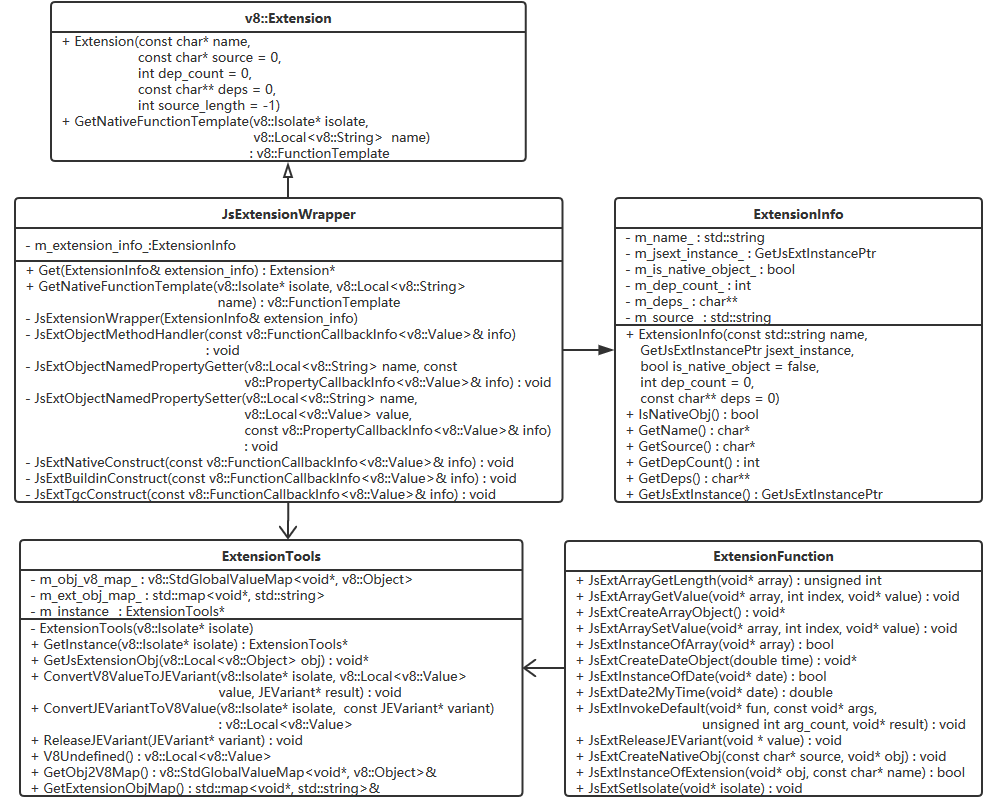
\includegraphics[width=\textwidth]{image/extension_framework/extension_framework_class.png} 
  \caption{extension framwork静态类图} \label{fig:extension_framework_class} 
\end{figure}

如第图~\ref{fig:extension_framework_class}所示:
v8扩展机制主要是继承v8内置的Extension类,通过重写其GetNativeFunctionTemplate方法来获取FunctionTemplate对象;
JsExtensionWrapper类主要就是封装创建出来的FunctionTemplate对象的一些特性,比如构造函数,属性拦截器,方法执行;
ExtensionInfo类主要记录了创建v8扩展所有需要的关键信息;ExtensionTools类主要是提供简易的函数,比如通过v8::Object类获取ExtensionBase对象,
将v8变量转换为扩展变量,将扩展变量转换为v8变量,释放扩展变量等;ExtensionFunction主要提供常用对外接口给js扩展调用。

\begin{figure}[H] 
  \centering 
  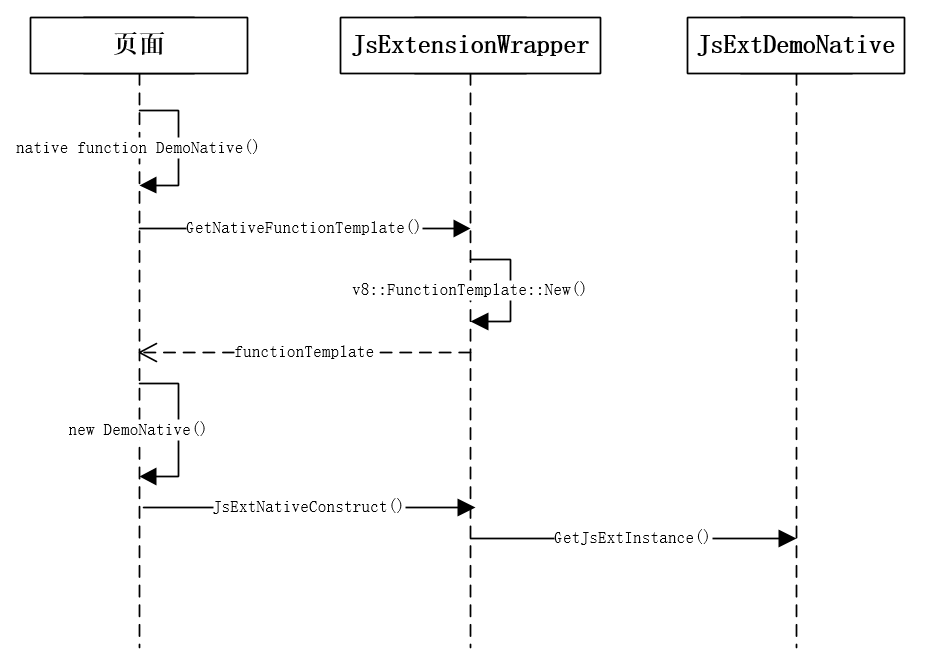
\includegraphics[width=\textwidth]{image/extension_framework/extension_construct_sequence.png} 
  \caption{js扩展对象创建时序图} \label{fig:extension_construct_sequence} 
\end{figure}

js扩展对象创建时序图如图~\ref{fig:extension_construct_sequence}所示:
\begin{itemize}
  \item 在页面加载时,v8::extension会注入页面代码native function DemoNative(),此时v8就会去创建DemoNative对应functionTemplate模板类。
  \item 当web开发人员在页面使用new DemoNative()时,functionTemplate模板类就会返回一个v8::Object实例对象给页面。
  \item 同理,针对内置对象,v8::extension会注入页面代码native function DemoBuildin()和var DemoBuildin = DemoBuildin()两段代码,
  此时由于DemoBuildin变量覆盖了DemoBuildin方法名,所以只能通过DemoBuildin执行对应方法和函数,不能再被new。
\end{itemize}

\begin{figure}[H] 
  \centering 
  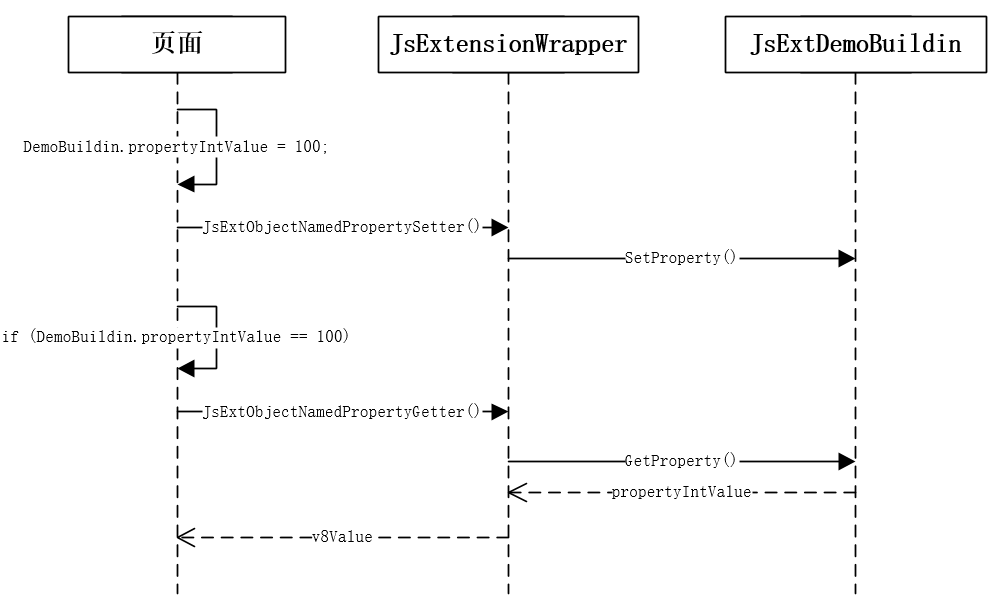
\includegraphics[width=\textwidth]{image/extension_framework/extension_property_sequence.png} 
  \caption{js扩展对象属性访问时序图} \label{fig:extension_property_sequence} 
\end{figure}

js扩展对象属性访问时序图如图~\ref{fig:extension_property_sequence}所示:
\begin{itemize}
  \item 由于在创建DemoBuildin对象时,对其ObjectTemplate模板类设置了拦截器特性,所以任何属性访问都会调用到拦截器的回调方法里。
\end{itemize}

\begin{figure}[H] 
  \centering 
  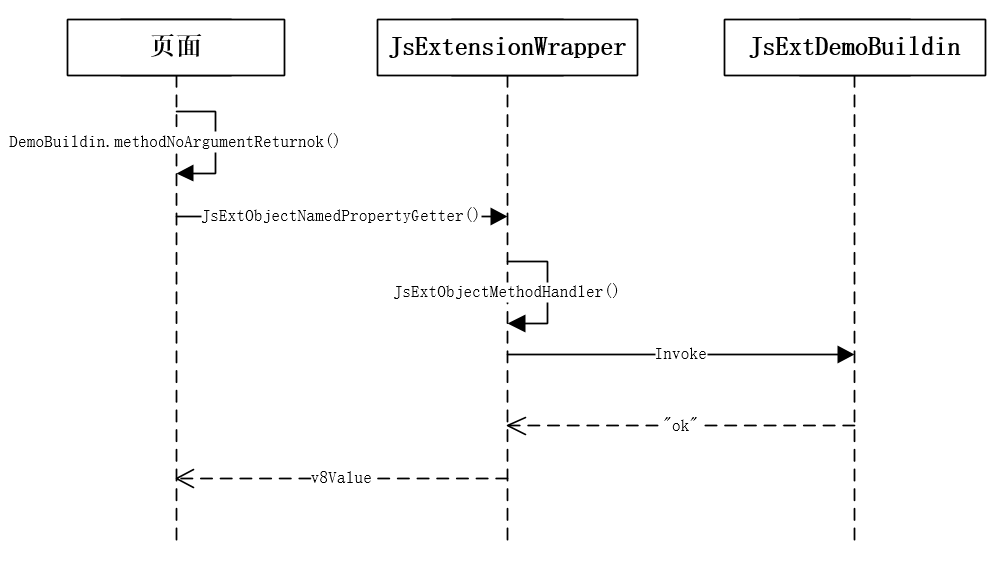
\includegraphics[width=\textwidth]{image/extension_framework/extension_function_sequence.png} 
  \caption{js扩展对象方法访问时序图} \label{fig:extension_function_sequence} 
\end{figure}

js扩展对象方法访问时序图如图~\ref{fig:extension_function_sequence}所示:
\begin{itemize}
  \item 同获取属性流程一致,当在拦截器回调函数里查询,如果属性没找到调用名,就去方法里找。
\end{itemize}

\section{Extension Framework垃圾回收机制}

对于内置对象,每次跳转页面,都会去调用其构造函数,此时回收机制的做法是先delete上个页面new出来的js扩展实例对象,再重新new一个js扩展实例对象,
然后绑定到v8 Object对象里。
\begin{spacing}{1.0}
\begin{lstlisting}[language={C++}]
void* delete_obj = ExtensionTools::GetJsExtensionObj(v8_obj);
  if (delete_obj) {
    ExtensionBase* ext_base = static_cast<ExtensionBase*>(delete_obj);
    delete ext_base;
    ext_base = NULL;
  }

  void* new_obj = NULL;
  extension_info->GetJsExtInstance()(NULL, 0, &new_obj);
  v8_obj->SetInternalField(ExtensionTools::JsExtBaseInternalField, v8::External::New(isolate, new_obj));
\end{lstlisting}
\end{spacing}

对于本地对象,每次创建对象时,我们会通过一个std::map保存js扩展实例对象指针以及name,当跳转页面,都会去调用tgc内置对象其构造函数,
将这个map里js扩展实例对象指针全部delete掉。
\begin{spacing}{1.0}
\begin{lstlisting}[language={C++}]
//在构造函数中将js扩展实例对象指针以及name保存到一个map中
void JsExtensionWrapper::JsExtNativeConstruct(const FunctionCallbackInfo<v8::Value>& info) {
  ...
  ExtensionTools* extension_tools = ExtensionTools::GetInstance(isolate);
  extension_tools->GetExtensionObjMap().insert(std::pair<void*, std::string>(new_obj, extension_info->GetName()));
  ...
}

//在tgc内置对象构造函数中将map中的js扩展实例对象指针全部delete掉
void JsExtensionWrapper::JsExtTgcConstruct(const FunctionCallbackInfo<v8::Value>& info) {
  ...
  ExtensionTools* extension_tools = ExtensionTools::GetInstance(isolate);
  std::map<void*, std::string>::iterator it;
  for (it = extension_tools->GetExtensionObjMap().begin(); it != extension_tools->GetExtensionObjMap().end(); it++) {
    ExtensionBase* ext_base = static_cast<ExtensionBase*>(it->first);
    if (ext_base) {
      delete ext_base;
      ext_base = NULL;
    }
  }
  ...
}
\end{lstlisting}
\end{spacing}



%---------------------------------------------------------------------

\ifx\withtbrowser\undefined
\else
\section{Extension Framework使用到的v8 API}

FunctionTemplate类是Function类的模板类,可以理解为设置Function的公共特性,
通过FunctionTemplate类new出来的Function类就拥有这些特性。相当于页面的function。
\begin{spacing}{1.0}
\begin{lstlisting}[language={C++}]
/**
@brief new一个FunctionTemplate对象

@param[in] isolate表示一个独立的v8引擎实例,每个实例维护不同的状态
@param[in] callback是回调函数,创建实例或方法被调用时会调用
@param[in] data表示给回调函数传递的额外的参数
@return 返回FunctionTemplate对象
*/
static Local<FunctionTemplate> New(
    Isolate* isolate, FunctionCallback callback = 0,
    Local<Value> data = Local<Value>(),
    Local<Signature> signature = Local<Signature>(), int length = 0,
    ConstructorBehavior behavior = ConstructorBehavior::kAllow);

/**
 * Set the call-handler callback for a FunctionTemplate.  This
 * callback is called whenever the function created from this
 * FunctionTemplate is called.
 */
void SetCallHandler(FunctionCallback callback,
    Local<Value> data = Local<Value>());
\end{lstlisting}
\end{spacing}

ObjectTemplate类是Object类的模板类,可以理解为设置Object的公共特性,
通过ObjectTemplate类new出来的Object类就拥有这些特性。相当于页面的object。
\begin{spacing}{1.0}
\begin{lstlisting}[language={C++}]
/**
@brief new一个ObjectTemplate对象

@param[in] isolate表示一个独立的v8引擎实例,每个实例维护不同的状态
@param[in] constructor是默认构造函数,只用于创建实例时会调用
@return 返回ObjectTemplate对象
*/
static Local<ObjectTemplate> New(
    Isolate* isolate,
    Local<FunctionTemplate> constructor = Local<FunctionTemplate>());

/**
@brief new一个Object对象实例

@param[in] context表示JavaScript代码运行环境上下文
@return 返回Object对象
*/
V8_WARN_UNUSED_RESULT MaybeLocal<Object> NewInstance(Local<Context> context);

/**
@brief 能够指定JavaScript访问对象属性时的一个callback

@param[in] getter表示获取属性时会被调用的callback
@param[in] setter表示设置属性时会被调用的callback
*/
void SetNamedPropertyHandler(NamedPropertyGetterCallback getter,
    NamedPropertySetterCallback setter = 0,
    NamedPropertyQueryCallback query = 0,
    NamedPropertyDeleterCallback deleter = 0,
    NamedPropertyEnumeratorCallback enumerator = 0,
    Local<Value> data = Local<Value>());
    
/**
@brief 通过这个模板生成的Object对象可以设置的内部field的数量

@param[in] value表示设置内部field的数量
*/
void SetInternalFieldCount(int value);
\end{lstlisting}
\end{spacing}

Object类是一个实例对象
\begin{spacing}{1.0}
\begin{lstlisting}[language={C++}]
/**
@brief 设置Object的内部field

@param[in] index表示Object的内部field的索引值,必须小于SetInternalFieldCount函数传入的值
@param[in] value表示Object的内部field值
*/
void SetInternalField(int index, Local<Value> value);
\end{lstlisting}
\end{spacing}

其他
\begin{spacing}{1.0}
\begin{lstlisting}[language={C++}]
/**
 * A map that uses Global as value and std::map as the backing
 * implementation. Globals are held non-weak.
 *
 * C++11 embedders don't need this class, as they can use
 * Global directly in std containers.
 */
template <typename K, typename V,
          typename Traits = DefaultGlobalMapTraits<K, V> >
class StdGlobalValueMap : public GlobalValueMap<K, V, Traits> {
 public:
  explicit StdGlobalValueMap(Isolate* isolate)
      : GlobalValueMap<K, V, Traits>(isolate) {}
};
\end{lstlisting}
\end{spacing}

\section{extension framework架构分析}
\begin{figure}[H] 
  \centering 
  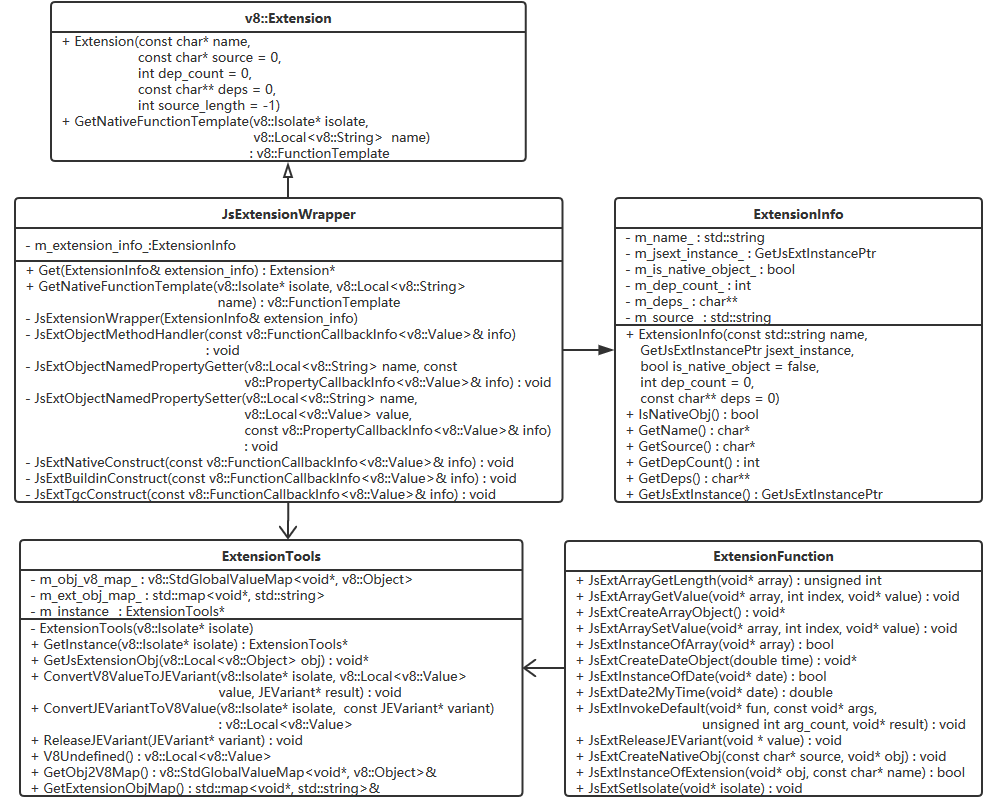
\includegraphics[width=\textwidth]{image/extension_framework/extension_framework_class.png} 
  \caption{extension framwork静态类图} \label{fig:extension_framework_class} 
\end{figure}

如第图~\ref{fig:extension_framework_class}所示:
v8扩展机制主要是继承v8内置的Extension类,通过重写其GetNativeFunctionTemplate方法来获取FunctionTemplate对象;
JsExtensionWrapper类主要就是封装创建出来的FunctionTemplate对象的一些特性,比如构造函数,属性拦截器,方法执行;
ExtensionInfo类主要记录了创建v8扩展所有需要的关键信息;ExtensionTools类主要是提供简易的函数,比如通过v8::Object类获取ExtensionBase对象,
将v8变量转换为扩展变量,将扩展变量转换为v8变量,释放扩展变量等;ExtensionFunction主要提供常用对外接口给js扩展调用。

\begin{figure}[H] 
  \centering 
  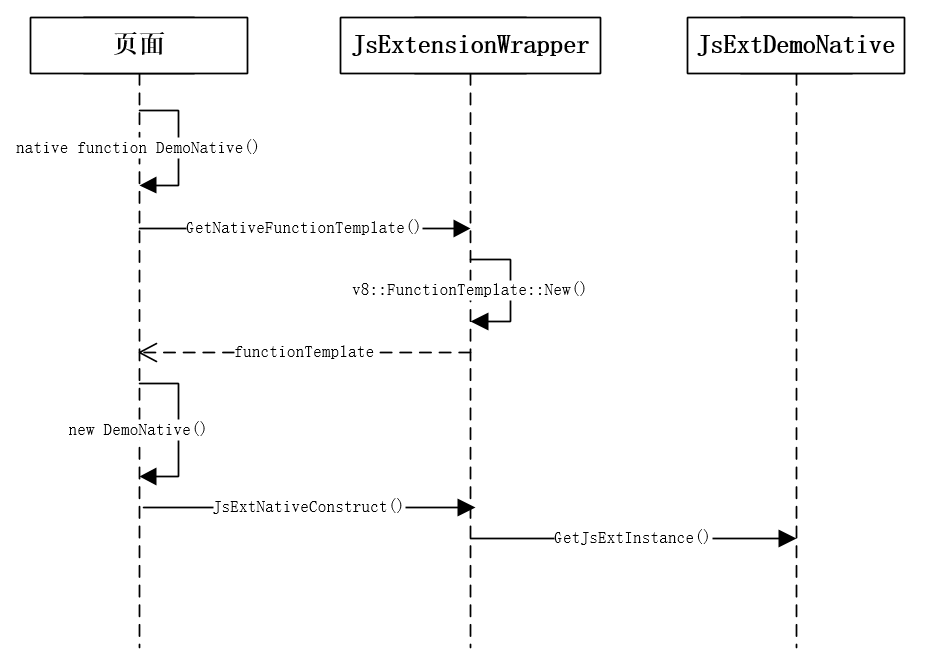
\includegraphics[width=\textwidth]{image/extension_framework/extension_construct_sequence.png} 
  \caption{js扩展对象创建时序图} \label{fig:extension_construct_sequence} 
\end{figure}

js扩展对象创建时序图如图~\ref{fig:extension_construct_sequence}所示:
\begin{itemize}
  \item 在页面加载时,v8::extension会注入页面代码native function DemoNative(),此时v8就会去创建DemoNative对应functionTemplate模板类。
  \item 当web开发人员在页面使用new DemoNative()时,functionTemplate模板类就会返回一个v8::Object实例对象给页面。
  \item 同理,针对内置对象,v8::extension会注入页面代码native function DemoBuildin()和var DemoBuildin = DemoBuildin()两段代码,
  此时由于DemoBuildin变量覆盖了DemoBuildin方法名,所以只能通过DemoBuildin执行对应方法和函数,不能再被new。
\end{itemize}

\begin{figure}[H] 
  \centering 
  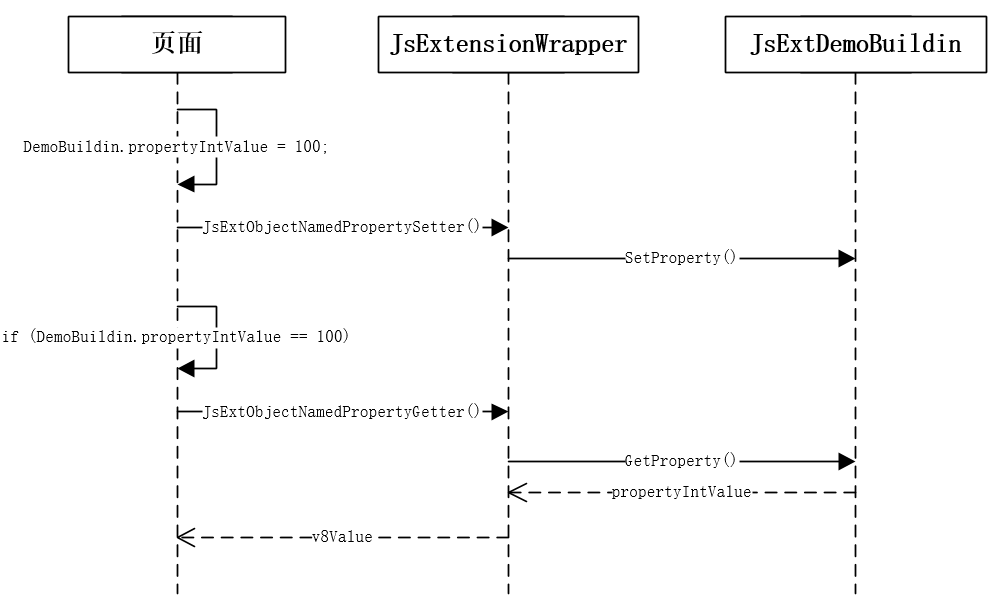
\includegraphics[width=\textwidth]{image/extension_framework/extension_property_sequence.png} 
  \caption{js扩展对象属性访问时序图} \label{fig:extension_property_sequence} 
\end{figure}

js扩展对象属性访问时序图如图~\ref{fig:extension_property_sequence}所示:
\begin{itemize}
  \item 由于在创建DemoBuildin对象时,对其ObjectTemplate模板类设置了拦截器特性,所以任何属性访问都会调用到拦截器的回调方法里。
\end{itemize}

\begin{figure}[H] 
  \centering 
  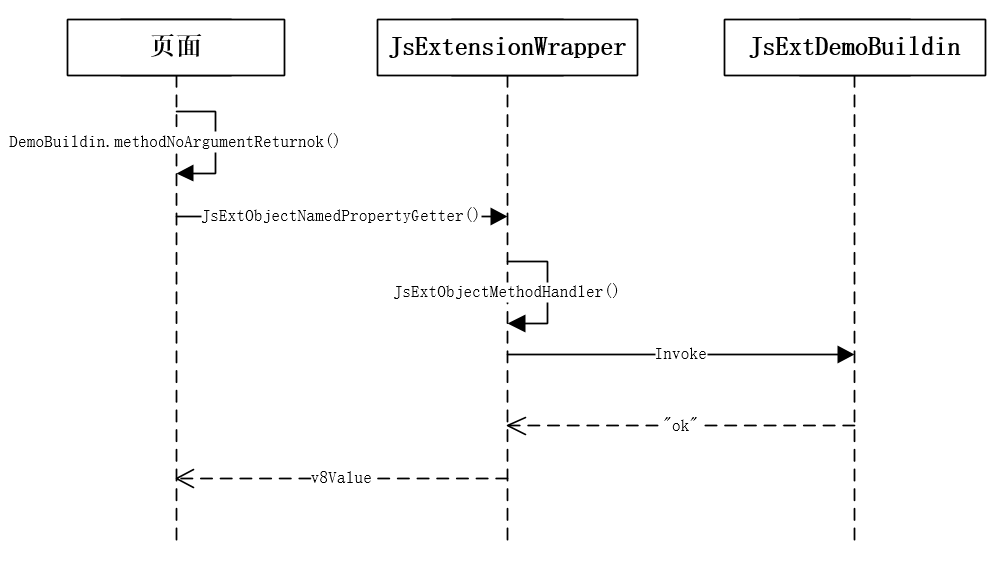
\includegraphics[width=\textwidth]{image/extension_framework/extension_function_sequence.png} 
  \caption{js扩展对象方法访问时序图} \label{fig:extension_function_sequence} 
\end{figure}

js扩展对象方法访问时序图如图~\ref{fig:extension_function_sequence}所示:
\begin{itemize}
  \item 同获取属性流程一致,当在拦截器回调函数里查询,如果属性没找到调用名,就去方法里找。
\end{itemize}

\section{Extension Framework垃圾回收机制}

对于内置对象,每次跳转页面,都会去调用其构造函数,此时回收机制的做法是先delete上个页面new出来的js扩展实例对象,再重新new一个js扩展实例对象,
然后绑定到v8 Object对象里。
\begin{spacing}{1.0}
\begin{lstlisting}[language={C++}]
void* delete_obj = ExtensionTools::GetJsExtensionObj(v8_obj);
  if (delete_obj) {
    ExtensionBase* ext_base = static_cast<ExtensionBase*>(delete_obj);
    delete ext_base;
    ext_base = NULL;
  }

  void* new_obj = NULL;
  extension_info->GetJsExtInstance()(NULL, 0, &new_obj);
  v8_obj->SetInternalField(ExtensionTools::JsExtBaseInternalField, v8::External::New(isolate, new_obj));
\end{lstlisting}
\end{spacing}

对于本地对象,每次创建对象时,我们会通过一个std::map保存js扩展实例对象指针以及name,当跳转页面,都会去调用tgc内置对象其构造函数,
将这个map里js扩展实例对象指针全部delete掉。
\begin{spacing}{1.0}
\begin{lstlisting}[language={C++}]
//在构造函数中将js扩展实例对象指针以及name保存到一个map中
void JsExtensionWrapper::JsExtNativeConstruct(const FunctionCallbackInfo<v8::Value>& info) {
  ...
  ExtensionTools* extension_tools = ExtensionTools::GetInstance(isolate);
  extension_tools->GetExtensionObjMap().insert(std::pair<void*, std::string>(new_obj, extension_info->GetName()));
  ...
}

//在tgc内置对象构造函数中将map中的js扩展实例对象指针全部delete掉
void JsExtensionWrapper::JsExtTgcConstruct(const FunctionCallbackInfo<v8::Value>& info) {
  ...
  ExtensionTools* extension_tools = ExtensionTools::GetInstance(isolate);
  std::map<void*, std::string>::iterator it;
  for (it = extension_tools->GetExtensionObjMap().begin(); it != extension_tools->GetExtensionObjMap().end(); it++) {
    ExtensionBase* ext_base = static_cast<ExtensionBase*>(it->first);
    if (ext_base) {
      delete ext_base;
      ext_base = NULL;
    }
  }
  ...
}
\end{lstlisting}
\end{spacing}



%---------------------------------------------------------------------

\ifx\withtbrowser\undefined
\else
\section{Extension Framework使用到的v8 API}

FunctionTemplate类是Function类的模板类,可以理解为设置Function的公共特性,
通过FunctionTemplate类new出来的Function类就拥有这些特性。相当于页面的function。
\begin{spacing}{1.0}
\begin{lstlisting}[language={C++}]
/**
@brief new一个FunctionTemplate对象

@param[in] isolate表示一个独立的v8引擎实例,每个实例维护不同的状态
@param[in] callback是回调函数,创建实例或方法被调用时会调用
@param[in] data表示给回调函数传递的额外的参数
@return 返回FunctionTemplate对象
*/
static Local<FunctionTemplate> New(
    Isolate* isolate, FunctionCallback callback = 0,
    Local<Value> data = Local<Value>(),
    Local<Signature> signature = Local<Signature>(), int length = 0,
    ConstructorBehavior behavior = ConstructorBehavior::kAllow);

/**
 * Set the call-handler callback for a FunctionTemplate.  This
 * callback is called whenever the function created from this
 * FunctionTemplate is called.
 */
void SetCallHandler(FunctionCallback callback,
    Local<Value> data = Local<Value>());
\end{lstlisting}
\end{spacing}

ObjectTemplate类是Object类的模板类,可以理解为设置Object的公共特性,
通过ObjectTemplate类new出来的Object类就拥有这些特性。相当于页面的object。
\begin{spacing}{1.0}
\begin{lstlisting}[language={C++}]
/**
@brief new一个ObjectTemplate对象

@param[in] isolate表示一个独立的v8引擎实例,每个实例维护不同的状态
@param[in] constructor是默认构造函数,只用于创建实例时会调用
@return 返回ObjectTemplate对象
*/
static Local<ObjectTemplate> New(
    Isolate* isolate,
    Local<FunctionTemplate> constructor = Local<FunctionTemplate>());

/**
@brief new一个Object对象实例

@param[in] context表示JavaScript代码运行环境上下文
@return 返回Object对象
*/
V8_WARN_UNUSED_RESULT MaybeLocal<Object> NewInstance(Local<Context> context);

/**
@brief 能够指定JavaScript访问对象属性时的一个callback

@param[in] getter表示获取属性时会被调用的callback
@param[in] setter表示设置属性时会被调用的callback
*/
void SetNamedPropertyHandler(NamedPropertyGetterCallback getter,
    NamedPropertySetterCallback setter = 0,
    NamedPropertyQueryCallback query = 0,
    NamedPropertyDeleterCallback deleter = 0,
    NamedPropertyEnumeratorCallback enumerator = 0,
    Local<Value> data = Local<Value>());
    
/**
@brief 通过这个模板生成的Object对象可以设置的内部field的数量

@param[in] value表示设置内部field的数量
*/
void SetInternalFieldCount(int value);
\end{lstlisting}
\end{spacing}

Object类是一个实例对象
\begin{spacing}{1.0}
\begin{lstlisting}[language={C++}]
/**
@brief 设置Object的内部field

@param[in] index表示Object的内部field的索引值,必须小于SetInternalFieldCount函数传入的值
@param[in] value表示Object的内部field值
*/
void SetInternalField(int index, Local<Value> value);
\end{lstlisting}
\end{spacing}

其他
\begin{spacing}{1.0}
\begin{lstlisting}[language={C++}]
/**
 * A map that uses Global as value and std::map as the backing
 * implementation. Globals are held non-weak.
 *
 * C++11 embedders don't need this class, as they can use
 * Global directly in std containers.
 */
template <typename K, typename V,
          typename Traits = DefaultGlobalMapTraits<K, V> >
class StdGlobalValueMap : public GlobalValueMap<K, V, Traits> {
 public:
  explicit StdGlobalValueMap(Isolate* isolate)
      : GlobalValueMap<K, V, Traits>(isolate) {}
};
\end{lstlisting}
\end{spacing}

\section{extension framework架构分析}
\begin{figure}[H] 
  \centering 
  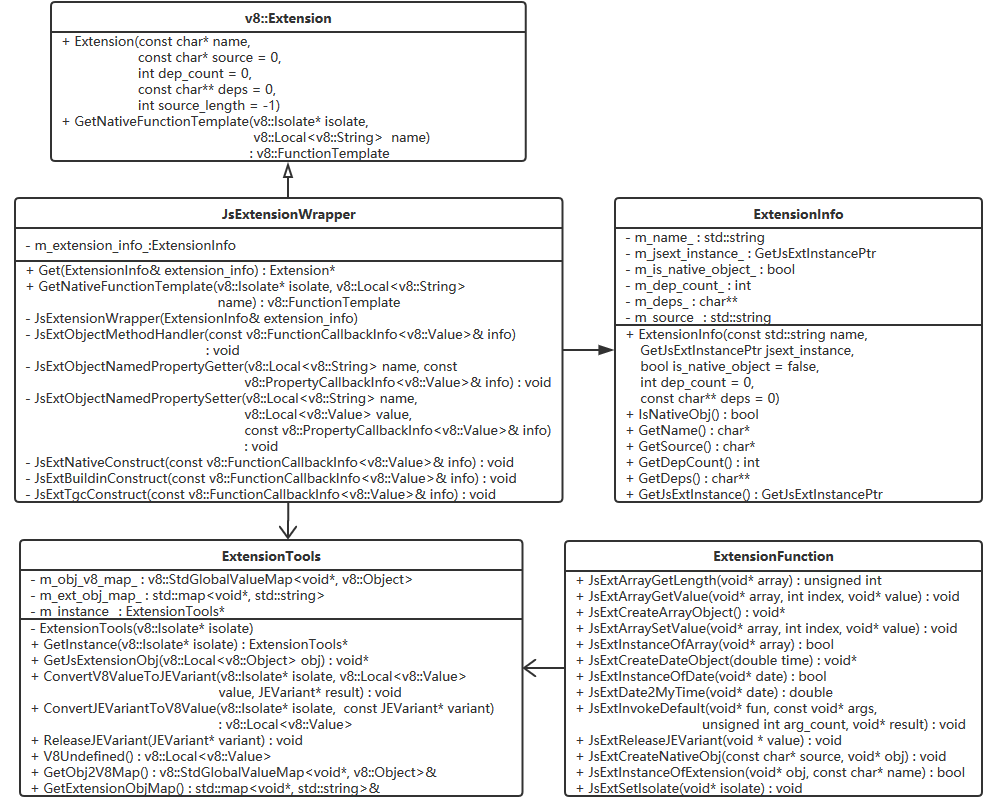
\includegraphics[width=\textwidth]{image/extension_framework/extension_framework_class.png} 
  \caption{extension framwork静态类图} \label{fig:extension_framework_class} 
\end{figure}

如第图~\ref{fig:extension_framework_class}所示:
v8扩展机制主要是继承v8内置的Extension类,通过重写其GetNativeFunctionTemplate方法来获取FunctionTemplate对象;
JsExtensionWrapper类主要就是封装创建出来的FunctionTemplate对象的一些特性,比如构造函数,属性拦截器,方法执行;
ExtensionInfo类主要记录了创建v8扩展所有需要的关键信息;ExtensionTools类主要是提供简易的函数,比如通过v8::Object类获取ExtensionBase对象,
将v8变量转换为扩展变量,将扩展变量转换为v8变量,释放扩展变量等;ExtensionFunction主要提供常用对外接口给js扩展调用。

\begin{figure}[H] 
  \centering 
  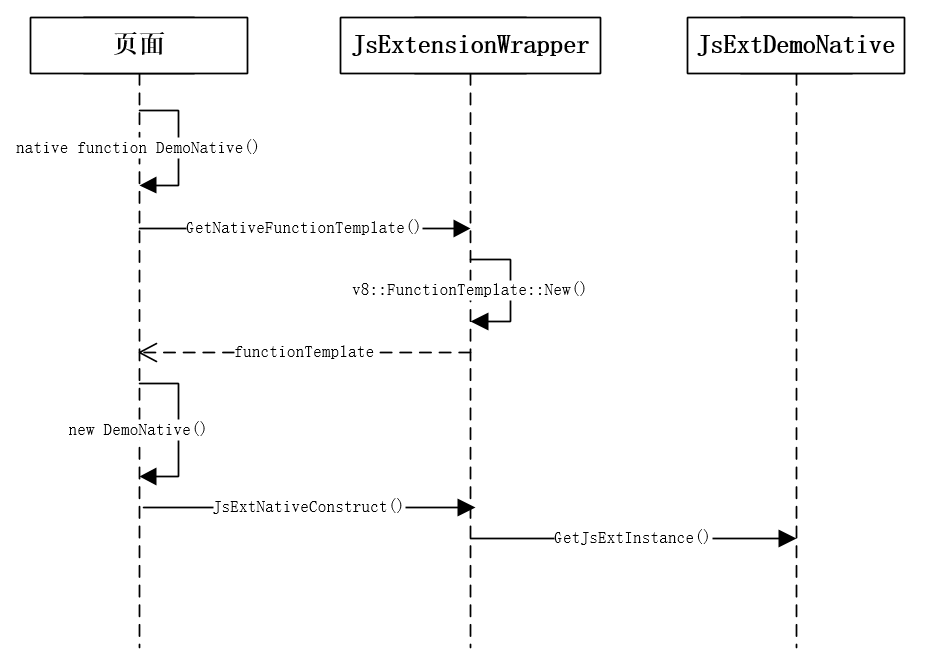
\includegraphics[width=\textwidth]{image/extension_framework/extension_construct_sequence.png} 
  \caption{js扩展对象创建时序图} \label{fig:extension_construct_sequence} 
\end{figure}

js扩展对象创建时序图如图~\ref{fig:extension_construct_sequence}所示:
\begin{itemize}
  \item 在页面加载时,v8::extension会注入页面代码native function DemoNative(),此时v8就会去创建DemoNative对应functionTemplate模板类。
  \item 当web开发人员在页面使用new DemoNative()时,functionTemplate模板类就会返回一个v8::Object实例对象给页面。
  \item 同理,针对内置对象,v8::extension会注入页面代码native function DemoBuildin()和var DemoBuildin = DemoBuildin()两段代码,
  此时由于DemoBuildin变量覆盖了DemoBuildin方法名,所以只能通过DemoBuildin执行对应方法和函数,不能再被new。
\end{itemize}

\begin{figure}[H] 
  \centering 
  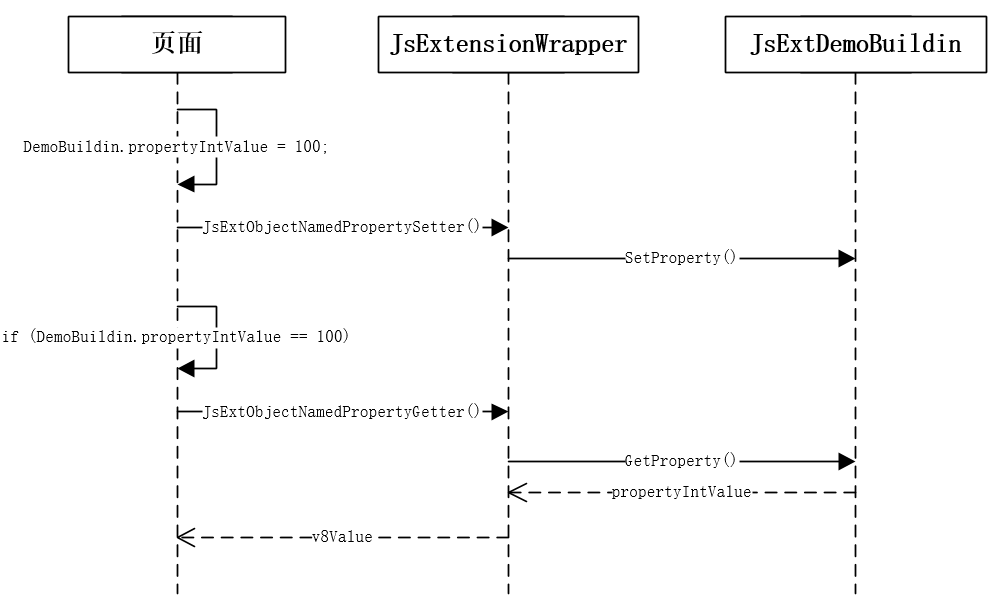
\includegraphics[width=\textwidth]{image/extension_framework/extension_property_sequence.png} 
  \caption{js扩展对象属性访问时序图} \label{fig:extension_property_sequence} 
\end{figure}

js扩展对象属性访问时序图如图~\ref{fig:extension_property_sequence}所示:
\begin{itemize}
  \item 由于在创建DemoBuildin对象时,对其ObjectTemplate模板类设置了拦截器特性,所以任何属性访问都会调用到拦截器的回调方法里。
\end{itemize}

\begin{figure}[H] 
  \centering 
  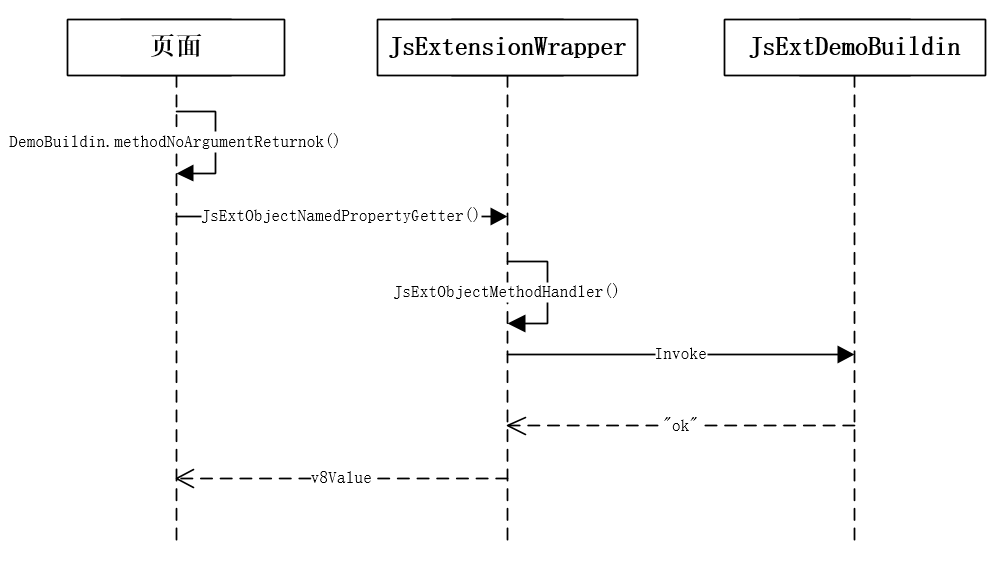
\includegraphics[width=\textwidth]{image/extension_framework/extension_function_sequence.png} 
  \caption{js扩展对象方法访问时序图} \label{fig:extension_function_sequence} 
\end{figure}

js扩展对象方法访问时序图如图~\ref{fig:extension_function_sequence}所示:
\begin{itemize}
  \item 同获取属性流程一致,当在拦截器回调函数里查询,如果属性没找到调用名,就去方法里找。
\end{itemize}

\section{Extension Framework垃圾回收机制}

对于内置对象,每次跳转页面,都会去调用其构造函数,此时回收机制的做法是先delete上个页面new出来的js扩展实例对象,再重新new一个js扩展实例对象,
然后绑定到v8 Object对象里。
\begin{spacing}{1.0}
\begin{lstlisting}[language={C++}]
void* delete_obj = ExtensionTools::GetJsExtensionObj(v8_obj);
  if (delete_obj) {
    ExtensionBase* ext_base = static_cast<ExtensionBase*>(delete_obj);
    delete ext_base;
    ext_base = NULL;
  }

  void* new_obj = NULL;
  extension_info->GetJsExtInstance()(NULL, 0, &new_obj);
  v8_obj->SetInternalField(ExtensionTools::JsExtBaseInternalField, v8::External::New(isolate, new_obj));
\end{lstlisting}
\end{spacing}

对于本地对象,每次创建对象时,我们会通过一个std::map保存js扩展实例对象指针以及name,当跳转页面,都会去调用tgc内置对象其构造函数,
将这个map里js扩展实例对象指针全部delete掉。
\begin{spacing}{1.0}
\begin{lstlisting}[language={C++}]
//在构造函数中将js扩展实例对象指针以及name保存到一个map中
void JsExtensionWrapper::JsExtNativeConstruct(const FunctionCallbackInfo<v8::Value>& info) {
  ...
  ExtensionTools* extension_tools = ExtensionTools::GetInstance(isolate);
  extension_tools->GetExtensionObjMap().insert(std::pair<void*, std::string>(new_obj, extension_info->GetName()));
  ...
}

//在tgc内置对象构造函数中将map中的js扩展实例对象指针全部delete掉
void JsExtensionWrapper::JsExtTgcConstruct(const FunctionCallbackInfo<v8::Value>& info) {
  ...
  ExtensionTools* extension_tools = ExtensionTools::GetInstance(isolate);
  std::map<void*, std::string>::iterator it;
  for (it = extension_tools->GetExtensionObjMap().begin(); it != extension_tools->GetExtensionObjMap().end(); it++) {
    ExtensionBase* ext_base = static_cast<ExtensionBase*>(it->first);
    if (ext_base) {
      delete ext_base;
      ext_base = NULL;
    }
  }
  ...
}
\end{lstlisting}
\end{spacing}



%---------------------------------------------------------------------

\ifx\withtbrowser\undefined
\else
\input{contents/extension_framework.tex}
\fi

\fi

\fi

\fi
